\documentclass{anstrans}
%%%%%%%%%%%%%%%%%%%%%%%%%%%%%%%%%%%
\title{%
The Nuclear Forensics Problem and Statistical Methods: \\
Evaluating Machine Learning for Spent Fuel Prediction
}
\author{Arrielle C. Opotowsky, Paul P.H. Wilson}

\institute{
Computational Nuclear Engineering Research Group \\
University of Wisconsin at Madison
}

\email{opotowsky@wisc.edu \and paulwilson@wisc.edu}

% Optional disclaimer: remove this command to hide
% \disclaimer{Notice: }

%%%% packages and definitions (optional)
\usepackage{graphicx} % allows inclusion of graphics
\usepackage{booktabs} % nice rules (thick lines) for tables
\usepackage{microtype} % improves typography for PDF

\newcommand{\SN}{S$_N$}
\renewcommand{\vec}[1]{\bm{#1}} %vector is bold italic
\newcommand{\vd}{\bm{\cdot}} % slightly bold vector dot
\newcommand{\grad}{\vec{\nabla}} % gradient
\newcommand{\ud}{\mathop{}\!\mathrm{d}} % upright derivative symbol

\begin{document}
%%%%%%%%%%%%%%%%%%%%%%%%%%%%%%%%%%%%%%%%%%%%%%%%%%%%%%%%%%%%%%%%%%%%%%%%%%%%%%%%
\section{Introduction}

In the event of a nuclear incident, such as the retrieval of stolen nuclear
material or the detonation of a dirty bomb, it is necessary to learn as much as
possible about the source of the materials in a timely manner. To characterize
the materials, both radiological methods (e.g., gamma spectroscopy) and
ionization methods (e.g., mass spectroscopy) are used to determine isotopic
ratios, chemical compounds, or trace elements. Although each category has a
multitude of techniques within it, the main tradeoff is between time/cost and
amount of information gained. 

The results of these analytic techniques are then compared against existing
databases to determine the origin of the nuclear material(s). These databases
are highly multidimensional, and furthermore, are rife with missing data
entries and inconsistent uncertainties. Direct comparison between measurement
results and a database therefore may not yield accurate results. Fortunately,
machine learning algorithms can be explored to create a model from a database
to "fill between the lines".  Additionally, having a machine-learned model may
overcome the above challenges of multidimensionality, missing data, and
irregular uncertainty.

While different machine learning algorithms and parameters will be
investigated, it is first important to determine if statistical methods can
overcome the inherent database deficiencies. Thus, this paper focuses on
probing the amount of information required to obtain realistic results.  This
can be best understood as the analgous real-world scenario.  Although mass
spectroscopy techniques provide extremely accurate isotopic information, they
are time-consuming and more expensice. And although gamma spectroscopy can give
extremely fast results cheaply, it only measures certain radiological signals
and is influenced by many environmental (or storage) factors. In the simulation
and machine learning paradigm, we need to determine what exactly is needed to
train a machine-learned model. Can the algorithm overcome the deficiencies of
gamma detection and still provide useful results? Or does it need more
information, e.g., exact isotopics?

Thus, ultimately, the goal is to answer the question \textit{How does the
ability to determine forensic-relevant spent nuclear fuel attributes degrade as
less information is available?}. But first, we must establish some baseline
expectations and algorithms to use. This work is based off previous work on the
subject (cite Dayman), and expands upon it by also evaluating a more advanced
machine learning algorithm: neural nets. Below is a more in depth discussion of
nuclear forensics and how machine learning can contribute to this research
area. After that, an experimental design is outlined. Lastly, the results are
presented and discussed. 

%%%%%%%%%%%%%%%%%%%%%%%%%%%%%%%%%%%%%%%%%%%%%%%%%%%%%%%%%%%%%%%%%%%%%%%%%%%%%%%%
\section{Background and Theory}

\subsection{Nuclear Forensics}

Nuclear forensics is the analysis and interpretation to determine the history
of nuclear material, whether that be intercepted spent nuclear fuel, uranium
ore concentrate, or the debris from an exploded nuclear device. Technical
nuclear forensics focuses on the characterization and interpretation of those
results. This, in combination with intelligence data, aids in material
attribution, which is the overall goal of nuclear forensics.  

Workflow for determining SNF quantities of interest: measure material, use
isotope content and/or isotope ratios to determine things like reactor type,
fuel type and enrichment at beginning of irradiation, cooling time, burnup.

After the material characteristics are measured, they are matched in a
forensics database that includes some or all this information for
pre-existing/pre-measured SNF. These databases are kept by individual
countries, and a given database will have widely varying uncertainty depending
where the material was measured as well as missing data in some fields.
Therefore, matching can be difficult.

(Classification, Characterization, Interpretation (Analysis), Reconstruction
(Attribution) - from the New Nuclear Forensics book) (Char methods to get
isotopic ratios or use S/ML, Interp examples)

To accomplish this, (we want to see if) it is possible to limit material
measurements to rapid-result nondestructive analysis, such as gamma ray
spectroscopy. Gamma spec gives less information at a higher uncertainty than
the near perfect results of some destructive mass spec techniques, like TIMS.
Additionally, within gamma spec techniques (field vs lab), uncertainties can
also vary.

(Something on goal to get as much info as possible within 24 h of interception
or device detonation). 

\subsection{Machine Learning}

Given imperfect data with varying amounts of uncertainty as well as the
required comparison to imperfect databases, many have begun considering
artificial intelligence approaches to nuclear forensics problems, such as
implementing searching algorithms for database comparison and machine learning
for determining spent fuel characteristics (cite all). A variety of statistical
and machine learning tools have been used to both classify spent fuel (reactor
type, fuel type) and predict values such as burnup, initial enrichment, or
cooling time (regression).

Add some real ML background here

%%%%%%%%%%%%%%%%%%%%%%%%%%%%%%%%%%%%%%%%%%%%%%%%%%%%%%%%%%%%%%%%%%%%%%%%%%%%%%%%
\section{Experimental Design}

This work begins by replicating the training and test sets used in ref (cite
Dayman). The study does evaluate the imapact of randomly introduced error of
varying amounts on the ability of the algorithms to correctly predict the
burnup and reactor type. It also varies the amount of nuclides given as
training to the algorithms (a full list, a short list determined by PCA, and
fission products only). However, machine learning algorithms are heavily
dependent on the inputs and parameters given to them, such as training set
sizes, learning rates, etc. Additionally, it does not consider more advanced
aglorithms. This paper adds in the comparison of the simpler algorithms to
neural nets. It also presents learning curves for each algorithm to investigate
the effect of the training set size on prediction error. For the classification
of reactor type, ROC curves are also presented to evaluate prediction and
generalization strength. For the regression of burnup, ??? pairwise t test?.
Thus, I will first investigate these algorithms with no error introduced, but
will extend the validation from a predetermined test set to be randomly
partitioned cross validation.  And the next study will introduce error by
limiting the nuclides to only those that can be measured with a gamma
spectrometer (future work).

\subsection{Algorithms Used}

NN classifier+regressor, ridge classification + regression, neural net
classification + regression- these are all discussed above, but can talk deets
+ parameters here

\subsection{Validation of Each Algorithm}

Using predetermined test set:

1. Learning curves: For a given (randomly chosen) training set size for each
algorithm, run several trainings and predictions. This helps determine if we
are over or under training and each algorithm's robustness to over/under
fitting.  

2. Classification Training Error: Precision/recall values / ROC curves for the
3 classes or maybe comparing algorithms to each other for each class

3. Regression Training Error: Confidence intervals on predictions to understand
true error versus sample error Test set must be > 30 instances, Can easily
calculate N\% confidence interval.

Using cross-validation instead:

1. redo learning curve study without having to run several trainings and
predictions for each set (bc that's already done!)

2. redo precision/recall study 

3. redo confidence interval study


\subsection{Comparing Algorithms}

Maybe can delete this if I already discuss it in the above section. Options for
comparison of algorithms: Comparing classification of 2 classes on same ROC
plot with multiple ML systems, Scatter plots, Pairwise t-tests. 

%%%%%%%%%%%%%%%%%%%%%%%%%%%%%%%%%%%%%%%%%%%%%%%%%%%%%%%%%%%%%%%%%%%%%%%%%%%%%%%%
\section{Results and Analysis}

So far, should include, with all 4 algorithms shown in each plot:
1. Learning curves  + CV curve
2. ROC plots + CV plot
3. Confidence interval tables + CV table

For the above categories in the validation section, can show plots directly
next to each other (for 1, 2, 3) to hopefully show that cross validation
provides better generalizability.  Future work would be to investigate the
number of cross validation folds. 

%%%%%%%%%%%%%%%%%%%%%%%%%%%%%%%%%%%%%%%%%%%%%%%%%%%%%%%%%%%%%%%%%%%%%%%%%%%%%%%%
%\subsection{Subsection Goes Here}
%The user must manually capitalize initial letters of a subsection heading.
%
%For those who like equations in their papers, \LaTeX\ is a good choice. Here is
%an equation for the Marshak diffusion boundary condition:
%\begin{equation} \label{eq:marshak}
%  4 J^- = \phi + 2 D \vec{n} \vd \grad \phi \,.
%\end{equation}
%If we so choose, we can effortlessly reference the equation later.
%
%Another paragraph starts with Eq.~\eqref{eq:marshak} and sets $J^-$ to zero, a
%vacuum boundary condition:
%\begin{equation*}
%  0 = \phi + \frac{2}{3} \frac{1}{\sigma} \vec{n} \vd \grad \phi \,.
%\end{equation*}
%The extrapolation distance is $2/3$. A more detailed asymptotic analysis yields
%an extrapolation distance of about $0.71045$.
%
%Figure~\ref{fig:voltage} shows how a plot might conceivably look in your
%document. Always place figures after they are referenced so as not to throw
%off the reader. You can use symbols and different line styles to help
%differentiate your results, especially if they are printed in black and white.
%Note how Fig.~\ref{fig:voltage} uses dashed lines \verb|--| for the exact
%solution, solid lines \verb|-| for the new method's solutions, and dotted lines
%\verb|:| for existing inaccurate methods.
%\begin{figure}[ht] % replace 't' with 'b' to force it to be on the bottom
%  \centering
%  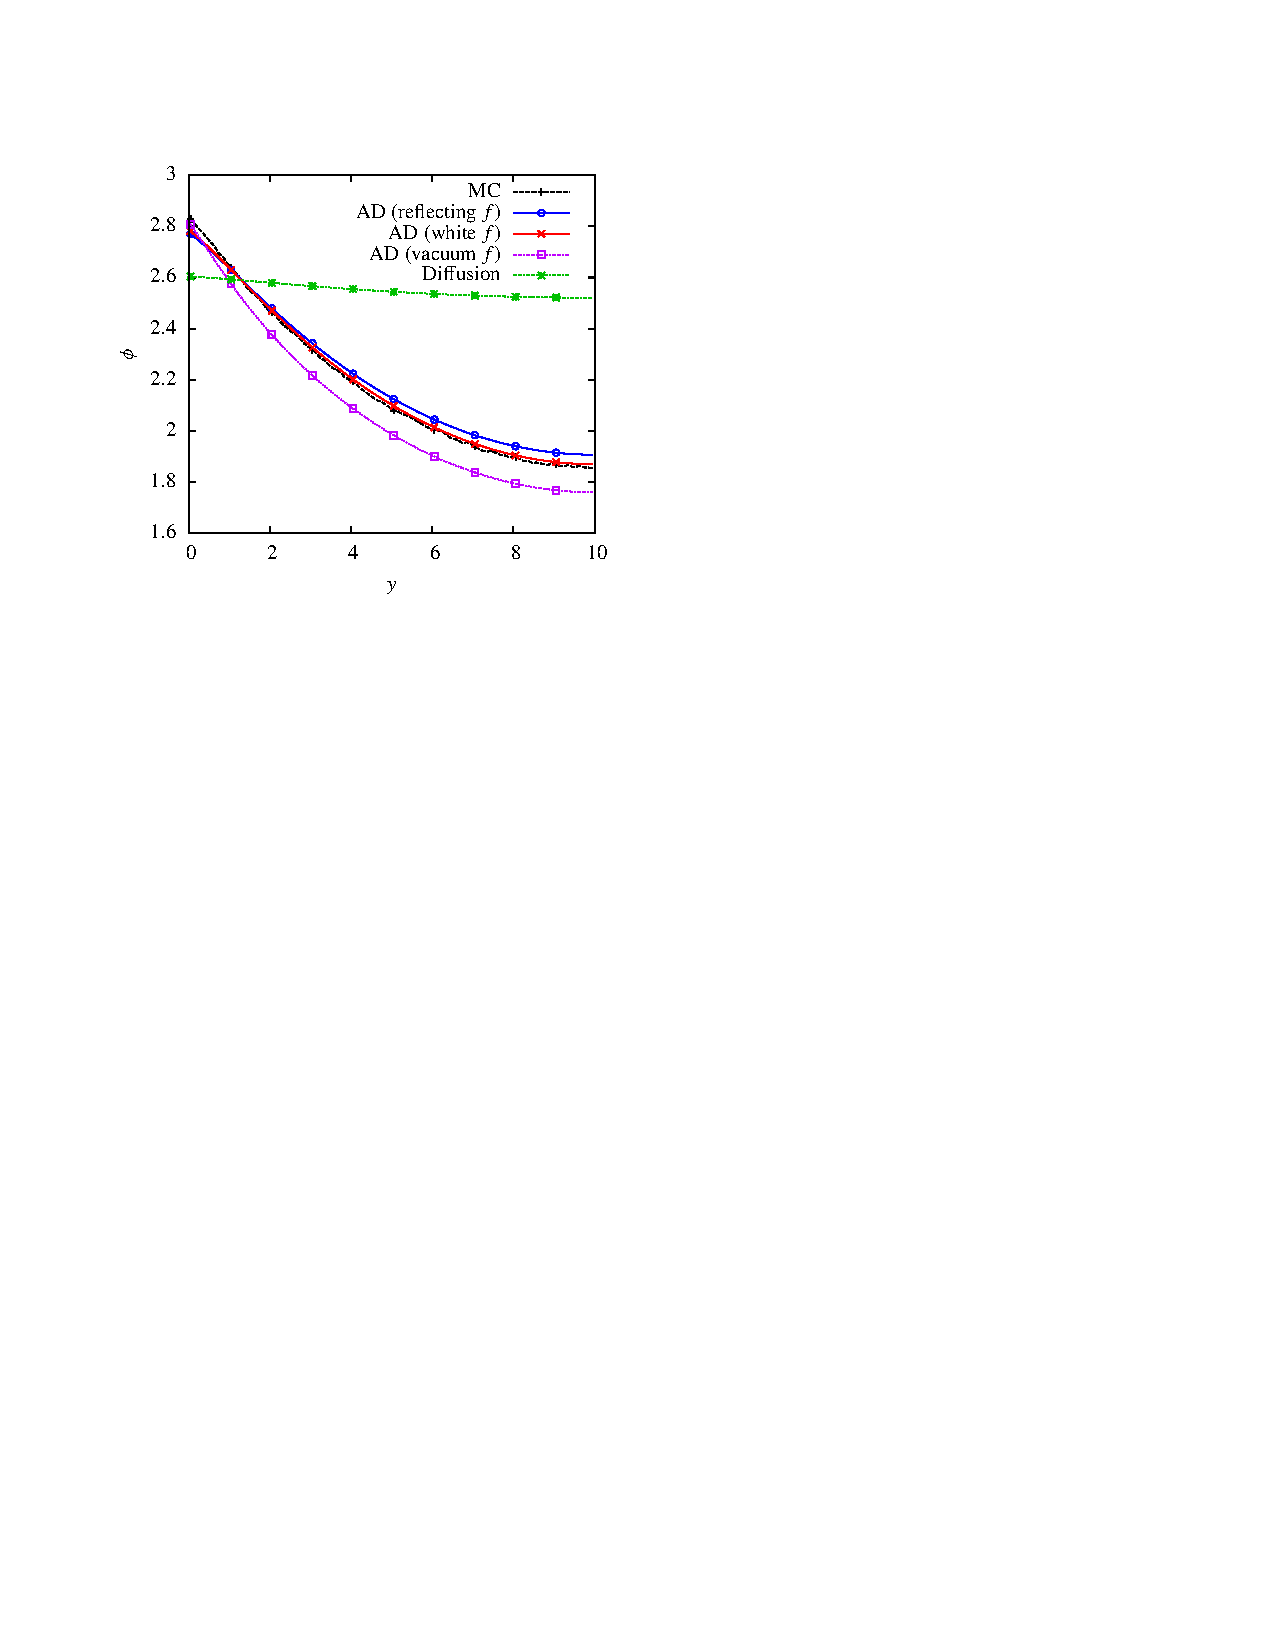
\includegraphics{example_figure}
%  \caption{Captions are flush with the left.}
%  \label{fig:voltage}
%\end{figure}
%
%Later on, we can include a table, even one that spans two columns such as
%Table~\ref{tab:widetable}.
%%%%%%%%%%%%%%%%%%%%%%%%%%%%%%%%%%%%%%%%%
%\begin{table*}[htb]
%  \centering
%\begin{tabular}{llllllllll}\toprule
%      & $\phi_T(0)$      & $\phi_T(10)$      & $\phi_T(20)$      &
%      $\phi_D(0)$      & $\phi_D(10)$      & $\phi_D(20)$      & $\rho$      &
%      $\varepsilon$      & $N_\text{it}$
%\\ \midrule
%$c=0.999$  & 0.9038 & 20.63 & 31.24 & 0.9087 & 20.63 & 31.23 & 0.2192 & $10^{-7}$ & 15
%\\
%$c=0.990$  & 0.3675 & 13.04 & 24.7 & 0.3696 & 13.04 & 24.69 & 0.2184 & $10^{-7}$ & 15
%\\
%$c=0.900$  & 0.009909 & 4.776 & 17.64 & 0.009984 & 4.786 & 17.63 & 0.2118 & $10^{-7}$ & 14
%\\
%$c=0.500$  & $6.069\times 10^{-5}$ & 2.212 & 15.53 & 6.213$\times 10^{-5}$ & 2.239 & 15.53 & 0.2068 & $10^{-7}$ & 13
%\\
%\bottomrule
%\end{tabular}
%  \caption{This is an example of a really wide table which might not normally
%  fit in the document.}
%  \label{tab:widetable}
%\end{table*}
%%%%%%%%%%%%%%%%%%%%%%%%%%%%%%%%%%%%%%%%%
%Notice how the table reference uses a Roman numeral
%for its numbering scheme, whereas the figure reference uses an Arabic numeral.
%For one-column tables, use the \verb|table| environment; two-column tables use
%\verb|table*|. The same applies to figures.
%
%%%%%%%%%%%%%%%%%%%%%%%%%%%%%%%%%%%%%%%%%%%%%%%%%%%%%%%%%%%%%%%%%%%%%%%%%%%%%%%%%
%\subsection{Another Subsection}
%Excessive sectioning in a three-page document is discouraged, but here are more
%subsections to demonstrate compliance with the ANS formatting guidelines.
%
%\subsubsection{Third-level Heading}
%This subsubsection shows compliance with the ANS-specified standard. This level
%of heading should be used rarely.
%
%\subsubsection{Another Such Heading}
%And, if you really think you need a third-level heading, you should make sure
%that your subsection needs at least two of them.
%
%%%%%%%%%%%%%%%%%%%%%%%%%%%%%%%%%%%%%%%%%%%%%%%%%%%%%%%%%%%%%%%%%%%%%%%%%%%%%%%%%
%\section{Conclusions}
%
%The included ANS style file and this clear example file are a panacea for
%the hours of headache that invariably results from formatting a document in
%Microsoft Word.
%
%%%%%%%%%%%%%%%%%%%%%%%%%%%%%%%%%%%%%%%%%%%%%%%%%%%%%%%%%%%%%%%%%%%%%%%%%%%%%%%%%
%\appendix
%\section{Appendix}
%
%Numbering in the appendix is different:
%\begin{equation} \label{eq:appendix}
%  2 + 2 = 5\,.
%\end{equation}
%and another equation:
%\begin{equation} \label{eq:appendix2}
%  a + b = c\,.
%\end{equation}

%%%%%%%%%%%%%%%%%%%%%%%%%%%%%%%%%%%%%%%%%%%%%%%%%%%%%%%%%%%%%%%%%%%%%%%%%%%%%%%%
\section{Acknowledgments}
This material is based upon work supported a Department of Energy Nuclear
Energy University Programs Graduate Fellowship.

%%%%%%%%%%%%%%%%%%%%%%%%%%%%%%%%%%%%%%%%%%%%%%%%%%%%%%%%%%%%%%%%%%%%%%%%%%%%%%%%
\bibliographystyle{ans}
\bibliography{bibliography}
\end{document}

